% OLD
%\documentclass[11pt,compress,t,notes=noshow, aspectratio=169, xcolor=table]{beamer}
% new
\documentclass[10pt,compress,t,notes=noshow, xcolor=table]{beamer}

% OLD
%\usepackage{../../style/lmu-lecture}
% new
\usepackage[]{graphicx}
% graphicx is loaded via lmu-lecture.sty as well
\usepackage[]{color}
% maxwidth is the original width if it is less than linewidth
% otherwise use linewidth (to make sure the graphics do not exceed the margin)
\makeatletter
\def\maxwidth{ %
  \ifdim\Gin@nat@width>\linewidth
    \linewidth
  \else
    \Gin@nat@width
  \fi
}
\makeatother

% ---------------------------------%
% latex-math dependencies, do not remove:
% - mathtools
% - bm
% - siunitx
% - dsfont
% - xspace
% ---------------------------------%

%--------------------------------------------------------%
%       Language, encoding, typography
%--------------------------------------------------------%

\usepackage[english]{babel}
\usepackage[utf8]{inputenc} % Enables inputting UTF-8 symbols
% Standard AMS suite (loaded via lmu-lecture.sty)
\usepackage{amsmath,amsfonts,amssymb}

% Font for double-stroke / blackboard letters for sets of numbers (N, R, ...)
% Distribution name is "doublestroke"
% According to https://mirror.physik.tu-berlin.de/pub/CTAN/fonts/doublestroke/dsdoc.pdf
% the "bbm" package does a similar thing and may be superfluous.
% Required for latex-math
\usepackage{dsfont}

% bbm – "Blackboard-style" cm fonts (https://www.ctan.org/pkg/bbm)
% Used to be in common.tex, loaded directly after this file
% Maybe superfluous given dsfont is loaded
% TODO: Check if really unused?
% \usepackage{bbm}

% bm – Access bold symbols in maths mode - https://ctan.org/pkg/bm
% Required for latex-math, preferred over \boldsymbol
% https://tex.stackexchange.com/questions/3238/bm-package-versus-boldsymbol
\usepackage{bm}

% pifont – Access to PostScript standard Symbol and Dingbats fonts
% Used for \newcommand{\xmark}{\ding{55}, which is never used
% aside from lecture_advml/attic/xx-automl/slides.Rnw
% \usepackage{pifont}

% Quotes (inline and display), provdes \enquote
% https://ctan.org/pkg/csquotes
\usepackage{csquotes}

% Adds arg to enumerate env, technically superseded by enumitem according
% to https://ctan.org/pkg/enumerate
% Replace with https://ctan.org/pkg/enumitem ?
% Even better: enumitem is not really compatible with beamer and breaks all sorts of things
% particularly the enumerate environment. The enumerate package also just isn't required
% from what I can tell so... don't re-add it I guess?
% \usepackage{enumerate}

% Line spacing - provides \singlespacing \doublespacing \onehalfspacing
% https://ctan.org/pkg/setspace
% \usepackage{setspace}

% mathtools – Mathematical tools to use with amsmath
% https://ctan.org/pkg/mathtools?lang=en
% latex-math dependency according to latex-math repo
\usepackage{mathtools}

% Maybe not great to use this https://tex.stackexchange.com/a/197/19093
% Use align instead -- TODO: Global search & replace to check, eqnarray is used a lot
% $ rg -f -u "\begin{eqnarray" -l | grep -v attic | awk -F '/' '{print $1}' | sort | uniq -c
%   13 lecture_advml
%   14 lecture_i2ml
%    2 lecture_iml
%   27 lecture_optimization
%   45 lecture_sl
\usepackage{eqnarray}

% For shaded regions / boxes
% Used sometimes in optim
% https://www.ctan.org/pkg/framed
\usepackage{framed}

%--------------------------------------------------------%
%       Cite button (version 2024-05)
%--------------------------------------------------------%
% Note this requires biber to be in $PATH when running,
% telltale error in log would be e.g. Package biblatex Info: ... file 'authoryear.dbx' not found
% aside from obvious "biber: command not found" or similar.
% Tried moving this to lmu-lecture.sty but had issues I didn't quite understood,
% so it's here for now.

\usepackage{textcase} % for \NoCaseChange
\usepackage{hyperref}

% Only try adding a references file if it exists, otherwise
% this would compile error when references.bib is not found
\IfFileExists{references.bib} {
  \usepackage{usebib}
  \usepackage[backend=biber, style=authoryear]{biblatex}

  \addbibresource{./references.bib}
  \bibinput{references}
}

\newcommand{\citelink}[1]{%
\NoCaseChange{\resizebox{!}{9pt}{\protect\beamergotobutton{\href{\usebibentry{\NoCaseChange{#1}}{url}}{\begin{NoHyper}\cite{#1}\end{NoHyper}}}}}%
}

%--------------------------------------------------------%
%       Displaying code and algorithms
%--------------------------------------------------------%

% Reimplements verbatim environments: https://ctan.org/pkg/verbatim
% verbatim used sed at least once in
% supervised-classification/slides-classification-tasks.tex
% Removed since code should not be put on slides anyway
% \usepackage{verbatim}

% Both used together for algorithm typesetting, see also overleaf: https://www.overleaf.com/learn/latex/Algorithms
% algorithmic env is also used, but part of the bundle:
%   "algpseudocode is part of the algorithmicx bundle, it gives you an improved version of algorithmic besides providing some other features"
% According to https://tex.stackexchange.com/questions/229355/algorithm-algorithmic-algorithmicx-algorithm2e-algpseudocode-confused
\usepackage{algorithm}
\usepackage{algpseudocode}

%--------------------------------------------------------%
%       Tables
%--------------------------------------------------------%

% multi-row table cells: https://www.namsu.de/Extra/pakete/Multirow.html
% Provides \multirow
% Used e.g. in evaluation/slides-evaluation-measures-classification.tex
\usepackage{multirow}

% colortbl: https://ctan.org/pkg/colortbl
% "The package allows rows and columns to be coloured, and even individual cells." well.
% Provides \columncolor and \rowcolor
% \rowcolor is used multiple times, e.g. in knn/slides-knn.tex
\usepackage{colortbl}

% long/multi-page tables: https://texdoc.org/serve/longtable.pdf/0
% Not used in slides
% \usepackage{longtable}

% pretty table env: https://ctan.org/pkg/booktabs
% Is used
% Defines \toprule
\usepackage{booktabs}

%--------------------------------------------------------%
%       Figures: Creating, placing, verbing
%--------------------------------------------------------%

% wrapfig - Wrapping text around figures https://de.overleaf.com/learn/latex/Wrapping_text_around_figures
% Provides wrapfigure environment -used in lecture_optimization
\usepackage{wrapfig}

% Sub figures in figures and tables
% https://ctan.org/pkg/subfig -- supersedes subfigure package
% Provides \subfigure
% \subfigure not used in slides but slides-tuning-practical.pdf errors without this pkg, error due to \captionsetup undefined
\usepackage{subfig}

% Actually it's pronounced PGF https://en.wikibooks.org/wiki/LaTeX/PGF/TikZ
\usepackage{tikz}

% No idea what/why these settings are what they are but I assume they're there on purpose
\usetikzlibrary{shapes,arrows,automata,positioning,calc,chains,trees, shadows}
\tikzset{
  %Define standard arrow tip
  >=stealth',
  %Define style for boxes
  punkt/.style={
    rectangle,
    rounded corners,
    draw=black, very thick,
    text width=6.5em,
    minimum height=2em,
    text centered},
  % Define arrow style
  pil/.style={
    ->,
    thick,
    shorten <=2pt,
    shorten >=2pt,}
}

%--------------------------------------------------------%
%       Beamer setup and custom macros & environments
%--------------------------------------------------------%

% Main sty file for beamer setup (layout, style, lecture page numbering, etc.)
% For long-term maintenance, this may me refactored into a more modular set of .sty files
\usepackage{../../style/lmu-lecture}
% Custom itemize wrappers, itemizeS, itemizeL, etc
\usepackage{../../style/customitemize}
% Custom framei environment, uses custom itemize!
\usepackage{../../style/framei}
% Custom frame2 environment, allows specifying font size for all content
\usepackage{../../style/frame2}
% Column layout macros
\usepackage{../../style/splitV} 

% Used regularly
\let\code=\texttt

% Not sure what/why this does
\setkeys{Gin}{width=0.9\textwidth}

% -- knitr leftovers --
% Used often in conjunction with \definecolor{shadecolor}{rgb}{0.969, 0.969, 0.969}
% Removing definitions requires chaning _many many_ slides, which then need checking to see if output still ok
\definecolor{fgcolor}{rgb}{0.345, 0.345, 0.345}
\definecolor{shadecolor}{rgb}{0.969, 0.969, 0.969}
\newenvironment{knitrout}{}{} % an empty environment to be redefined in TeX

%-------------------------------------------------------------------------------------------------------%
%  Unused stuff that needs to go but is kept here currently juuuust in case it was important after all  %
%-------------------------------------------------------------------------------------------------------%

% \newcommand{\hlnum}[1]{\textcolor[rgb]{0.686,0.059,0.569}{#1}}%
% \newcommand{\hlstr}[1]{\textcolor[rgb]{0.192,0.494,0.8}{#1}}%
% \newcommand{\hlcom}[1]{\textcolor[rgb]{0.678,0.584,0.686}{\textit{#1}}}%
% \newcommand{\hlopt}[1]{\textcolor[rgb]{0,0,0}{#1}}%
% \newcommand{\hlstd}[1]{\textcolor[rgb]{0.345,0.345,0.345}{#1}}%
% \newcommand{\hlkwa}[1]{\textcolor[rgb]{0.161,0.373,0.58}{\textbf{#1}}}%
% \newcommand{\hlkwb}[1]{\textcolor[rgb]{0.69,0.353,0.396}{#1}}%
% \newcommand{\hlkwc}[1]{\textcolor[rgb]{0.333,0.667,0.333}{#1}}%
% \newcommand{\hlkwd}[1]{\textcolor[rgb]{0.737,0.353,0.396}{\textbf{#1}}}%
% \let\hlipl\hlkwb

% \makeatletter
% \newenvironment{kframe}{%
%  \def\at@end@of@kframe{}%
%  \ifinner\ifhmode%
%   \def\at@end@of@kframe{\end{minipage}}%
%   \begin{minipage}{\columnwidth}%
%  \fi\fi%
%  \def\FrameCommand##1{\hskip\@totalleftmargin \hskip-\fboxsep
%  \colorbox{shadecolor}{##1}\hskip-\fboxsep
%      % There is no \\@totalrightmargin, so:
%      \hskip-\linewidth \hskip-\@totalleftmargin \hskip\columnwidth}%
%  \MakeFramed {\advance\hsize-\width
%    \@totalleftmargin\z@ \linewidth\hsize
%    \@setminipage}}%
%  {\par\unskip\endMakeFramed%
%  \at@end@of@kframe}
% \makeatother

% \definecolor{shadecolor}{rgb}{.97, .97, .97}
% \definecolor{messagecolor}{rgb}{0, 0, 0}
% \definecolor{warningcolor}{rgb}{1, 0, 1}
% \definecolor{errorcolor}{rgb}{1, 0, 0}
% \newenvironment{knitrout}{}{} % an empty environment to be redefined in TeX

% \usepackage{alltt}
% \newcommand{\SweaveOpts}[1]{}  % do not interfere with LaTeX
% \newcommand{\SweaveInput}[1]{} % because they are not real TeX commands
% \newcommand{\Sexpr}[1]{}       % will only be parsed by R
% \newcommand{\xmark}{\ding{55}}%

% textpos – Place boxes at arbitrary positions on the LATEX page
% https://ctan.org/pkg/textpos
% Provides \begin{textblock}
% TODO: Check if really unused?
% \usepackage[absolute,overlay]{textpos}

% -----------------------%
% Likely knitr leftovers %
% -----------------------%

% psfrag – Replace strings in encapsulated PostScript figures
% https://www.overleaf.com/latex/examples/psfrag-example/tggxhgzwrzhn
% https://ftp.mpi-inf.mpg.de/pub/tex/mirror/ftp.dante.de/pub/tex/macros/latex/contrib/psfrag/pfgguide.pdf
% Can't tell if this is needed
% TODO: Check if really unused?
% \usepackage{psfrag}

% arydshln – Draw dash-lines in array/tabular
% https://www.ctan.org/pkg/arydshln
% !! "arydshln has to be loaded after array, longtable, colortab and/or colortbl"
% Provides \hdashline and \cdashline
% Not used in slides
% \usepackage{arydshln}

% tabularx – Tabulars with adjustable-width columns
% https://ctan.org/pkg/tabularx
% Provides \begin{tabularx}
% Not used in slides
% \usepackage{tabularx}

% placeins – Control float placement
% https://ctan.org/pkg/placeins
% Defines a \FloatBarrier command
% TODO: Check if really unused?
% \usepackage{placeins}

% Can't find a reason why common.tex is not just part of this file?
% This file is included in slides and exercises

% Rarely used fontstyle for R packages, used only in 
% - forests/slides-forests-benchmark.tex
% - exercises/single-exercises/methods_l_1.Rnw
% - slides/cart/attic/slides_extra_trees.Rnw
\newcommand{\pkg}[1]{{\fontseries{b}\selectfont #1}}

% Spacing helpers, used often (mostly in exercises for \dlz)
\newcommand{\lz}{\vspace{0.5cm}} % vertical space (used often in slides)
\newcommand{\dlz}{\vspace{1cm}}  % double vertical space (used often in exercises, never in slides)
\newcommand{\oneliner}[1] % Oneliner for important statements, used e.g. in iml, algods
{\begin{block}{}\begin{center}\begin{Large}#1\end{Large}\end{center}\end{block}}

% Don't know if this is used or needed, remove?
% textcolor that works in mathmode
% https://tex.stackexchange.com/a/261480
% Used e.g. in forests/slides-forests-bagging.tex
% [...] \textcolor{blue}{\tfrac{1}{M}\sum^M_{m} [...]
% \makeatletter
% \renewcommand*{\@textcolor}[3]{%
%   \protect\leavevmode
%   \begingroup
%     \color#1{#2}#3%
%   \endgroup
% }
% \makeatother


% Defines macros and environments
 % machine learning
\newcommand{\Xspace}{\mathcal{X}} % X, input space
\newcommand{\Yspace}{\mathcal{Y}} % Y, output space
\newcommand{\Zspace}{\mathcal{Z}} % Z, space of sampled datapoints
\newcommand{\nset}{\{1, \ldots, n\}} % set from 1 to n
\newcommand{\pset}{\{1, \ldots, p\}} % set from 1 to p
\newcommand{\gset}{\{1, \ldots, g\}} % set from 1 to g
\newcommand{\Pxy}{\mathbb{P}_{xy}} % P_xy
\newcommand{\Exy}{\mathbb{E}_{xy}} % E_xy: Expectation over random variables xy
\newcommand{\xv}{\mathbf{x}} % vector x (bold)
\newcommand{\xtil}{\tilde{\mathbf{x}}} % vector x-tilde (bold)
\newcommand{\yv}{\mathbf{y}} % vector y (bold)
\newcommand{\xy}{(\xv, y)} % observation (x, y)
\newcommand{\xvec}{\left(x_1, \ldots, x_p\right)^\top} % (x1, ..., xp)
\newcommand{\Xmat}{\mathbf{X}} % Design matrix
\newcommand{\allDatasets}{\mathds{D}} % The set of all datasets
\newcommand{\allDatasetsn}{\mathds{D}_n}  % The set of all datasets of size n
\newcommand{\D}{\mathcal{D}} % D, data
\newcommand{\Dn}{\D_n} % D_n, data of size n
\newcommand{\Dtrain}{\mathcal{D}_{\text{train}}} % D_train, training set
\newcommand{\Dtest}{\mathcal{D}_{\text{test}}} % D_test, test set
\newcommand{\xyi}[1][i]{\left(\xv^{(#1)}, y^{(#1)}\right)} % (x^i, y^i), i-th observation
\newcommand{\Dset}{\left( \xyi[1], \ldots, \xyi[n]\right)} % {(x1,y1)), ..., (xn,yn)}, data
\newcommand{\defAllDatasetsn}{(\Xspace \times \Yspace)^n} % Def. of the set of all datasets of size n
\newcommand{\defAllDatasets}{\bigcup_{n \in \N}(\Xspace \times \Yspace)^n} % Def. of the set of all datasets
\newcommand{\xdat}{\left\{ \xv^{(1)}, \ldots, \xv^{(n)}\right\}} % {x1, ..., xn}, input data
\newcommand{\ydat}{\left\{ \yv^{(1)}, \ldots, \yv^{(n)}\right\}} % {y1, ..., yn}, input data
\newcommand{\yvec}{\left(y^{(1)}, \hdots, y^{(n)}\right)^\top} % (y1, ..., yn), vector of outcomes
\newcommand{\greekxi}{\xi} % Greek letter xi
\renewcommand{\xi}[1][i]{\xv^{(#1)}} % x^i, i-th observed value of x
\newcommand{\yi}[1][i]{y^{(#1)}} % y^i, i-th observed value of y
\newcommand{\xivec}{\left(x^{(i)}_1, \ldots, x^{(i)}_p\right)^\top} % (x1^i, ..., xp^i), i-th observation vector
\newcommand{\xj}{\xv_j} % x_j, j-th feature
\newcommand{\xjvec}{\left(x^{(1)}_j, \ldots, x^{(n)}_j\right)^\top} % (x^1_j, ..., x^n_j), j-th feature vector
\newcommand{\phiv}{\mathbf{\phi}} % Basis transformation function phi
\newcommand{\phixi}{\mathbf{\phi}^{(i)}} % Basis transformation of xi: phi^i := phi(xi)

%%%%%% ml - models general
\newcommand{\lamv}{\bm{\lambda}} % lambda vector, hyperconfiguration vector
\newcommand{\Lam}{\bm{\Lambda}}	 % Lambda, space of all hpos
% Inducer / Inducing algorithm
\newcommand{\preimageInducer}{\left(\defAllDatasets\right)\times\Lam} % Set of all datasets times the hyperparameter space
\newcommand{\preimageInducerShort}{\allDatasets\times\Lam} % Set of all datasets times the hyperparameter space
% Inducer / Inducing algorithm
\newcommand{\ind}{\mathcal{I}} % Inducer, inducing algorithm, learning algorithm

% continuous prediction function f
\newcommand{\ftrue}{f_{\text{true}}}  % True underlying function (if a statistical model is assumed)
\newcommand{\ftruex}{\ftrue(\xv)} % True underlying function (if a statistical model is assumed)
\newcommand{\fx}{f(\xv)} % f(x), continuous prediction function
\newcommand{\fdomains}{f: \Xspace \rightarrow \R^g} % f with domain and co-domain
\newcommand{\Hspace}{\mathcal{H}} % hypothesis space where f is from
\newcommand{\fbayes}{f^{\ast}} % Bayes-optimal model
\newcommand{\fxbayes}{f^{\ast}(\xv)} % Bayes-optimal model
\newcommand{\fkx}[1][k]{f_{#1}(\xv)} % f_j(x), discriminant component function
\newcommand{\fh}{\hat{f}} % f hat, estimated prediction function
\newcommand{\fxh}{\fh(\xv)} % fhat(x)
\newcommand{\fxt}{f(\xv ~|~ \thetav)} % f(x | theta)
\newcommand{\fxi}{f\left(\xv^{(i)}\right)} % f(x^(i))
\newcommand{\fxih}{\hat{f}\left(\xv^{(i)}\right)} % f(x^(i))
\newcommand{\fxit}{f\left(\xv^{(i)} ~|~ \thetav\right)} % f(x^(i) | theta)
\newcommand{\fhD}{\fh_{\D}} % fhat_D, estimate of f based on D
\newcommand{\fhDtrain}{\fh_{\Dtrain}} % fhat_Dtrain, estimate of f based on D
\newcommand{\fhDnlam}{\fh_{\Dn, \lamv}} %model learned on Dn with hp lambda
\newcommand{\fhDlam}{\fh_{\D, \lamv}} %model learned on D with hp lambda
\newcommand{\fhDnlams}{\fh_{\Dn, \lamv^\ast}} %model learned on Dn with optimal hp lambda
\newcommand{\fhDlams}{\fh_{\D, \lamv^\ast}} %model learned on D with optimal hp lambda

% discrete prediction function h
\newcommand{\hx}{h(\xv)} % h(x), discrete prediction function
\newcommand{\hh}{\hat{h}} % h hat
\newcommand{\hxh}{\hat{h}(\xv)} % hhat(x)
\newcommand{\hxt}{h(\xv | \thetav)} % h(x | theta)
\newcommand{\hxi}{h\left(\xi\right)} % h(x^(i))
\newcommand{\hxit}{h\left(\xi ~|~ \thetav\right)} % h(x^(i) | theta)
\newcommand{\hbayes}{h^{\ast}} % Bayes-optimal classification model
\newcommand{\hxbayes}{h^{\ast}(\xv)} % Bayes-optimal classification model

% yhat
\newcommand{\yh}{\hat{y}} % yhat for prediction of target
\newcommand{\yih}{\hat{y}^{(i)}} % yhat^(i) for prediction of ith targiet
\newcommand{\resi}{\yi- \yih}

% theta
\newcommand{\thetah}{\hat{\theta}} % theta hat
\newcommand{\thetav}{\bm{\theta}} % theta vector
\newcommand{\thetavh}{\bm{\hat\theta}} % theta vector hat
\newcommand{\thetat}[1][t]{\thetav^{[#1]}} % theta^[t] in optimization
\newcommand{\thetatn}[1][t]{\thetav^{[#1 +1]}} % theta^[t+1] in optimization
\newcommand{\thetahDnlam}{\thetavh_{\Dn, \lamv}} %theta learned on Dn with hp lambda
\newcommand{\thetahDlam}{\thetavh_{\D, \lamv}} %theta learned on D with hp lambda
\newcommand{\mint}{\min_{\thetav \in \Theta}} % min problem theta
\newcommand{\argmint}{\argmin_{\thetav \in \Theta}} % argmin theta

% densities + probabilities
% pdf of x
\newcommand{\pdf}{p} % p
\newcommand{\pdfx}{p(\xv)} % p(x)
\newcommand{\pixt}{\pi(\xv~|~ \thetav)} % pi(x|theta), pdf of x given theta
\newcommand{\pixit}[1][i]{\pi\left(\xi[#1] ~|~ \thetav\right)} % pi(x^i|theta), pdf of x given theta
\newcommand{\pixii}[1][i]{\pi\left(\xi[#1]\right)} % pi(x^i), pdf of i-th x

% pdf of (x, y)
\newcommand{\pdfxy}{p(\xv,y)} % p(x, y)
\newcommand{\pdfxyt}{p(\xv, y ~|~ \thetav)} % p(x, y | theta)
\newcommand{\pdfxyit}{p\left(\xi, \yi ~|~ \thetav\right)} % p(x^(i), y^(i) | theta)

% pdf of x given y
\newcommand{\pdfxyk}[1][k]{p(\xv | y= #1)} % p(x | y = k)
\newcommand{\lpdfxyk}[1][k]{\log p(\xv | y= #1)} % log p(x | y = k)
\newcommand{\pdfxiyk}[1][k]{p\left(\xi | y= #1 \right)} % p(x^i | y = k)

% prior probabilities
\newcommand{\pik}[1][k]{\pi_{#1}} % pi_k, prior
\newcommand{\pih}{\hat{\pi}} % pi hat, estimated prior (binary classification)
\newcommand{\pikh}[1][k]{\hat{\pi}_{#1}} % pi_k hat, estimated prior
\newcommand{\lpik}[1][k]{\log \pi_{#1}} % log pi_k, log of the prior
\newcommand{\pit}{\pi(\thetav)} % Prior probability of parameter theta

% posterior probabilities
\newcommand{\post}{\P(y = 1 ~|~ \xv)} % P(y = 1 | x), post. prob for y=1
\newcommand{\postk}[1][k]{\P(y = #1 ~|~ \xv)} % P(y = k | y), post. prob for y=k
\newcommand{\pidomains}{\pi: \Xspace \rightarrow \unitint} % pi with domain and co-domain
\newcommand{\pibayes}{\pi^{\ast}} % Bayes-optimal classification model
\newcommand{\pixbayes}{\pi^{\ast}(\xv)} % Bayes-optimal classification model
\newcommand{\pix}{\pi(\xv)} % pi(x), P(y = 1 | x)
\newcommand{\piv}{\bm{\pi}} % pi, bold, as vector
\newcommand{\pikx}[1][k]{\pi_{#1}(\xv)} % pi_k(x), P(y = k | x)
\newcommand{\pikxt}[1][k]{\pi_{#1}(\xv ~|~ \thetav)} % pi_k(x | theta), P(y = k | x, theta)
\newcommand{\pixh}{\hat \pi(\xv)} % pi(x) hat, P(y = 1 | x) hat
\newcommand{\pikxh}[1][k]{\hat \pi_{#1}(\xv)} % pi_k(x) hat, P(y = k | x) hat
\newcommand{\pixih}{\hat \pi(\xi)} % pi(x^(i)) with hat
\newcommand{\pikxih}[1][k]{\hat \pi_{#1}(\xi)} % pi_k(x^(i)) with hat
\newcommand{\pdfygxt}{p(y ~|~\xv, \thetav)} % p(y | x, theta)
\newcommand{\pdfyigxit}{p\left(\yi ~|~\xi, \thetav\right)} % p(y^i |x^i, theta)
\newcommand{\lpdfygxt}{\log \pdfygxt } % log p(y | x, theta)
\newcommand{\lpdfyigxit}{\log \pdfyigxit} % log p(y^i |x^i, theta)

% probababilistic
\newcommand{\bayesrulek}[1][k]{\frac{\P(\xv | y= #1) \P(y= #1)}{\P(\xv)}} % Bayes rule
\newcommand{\muv}{\bm{\mu}} % expectation vector of Gaussian
\newcommand{\muk}[1][k]{\bm{\mu_{#1}}} % mean vector of class-k Gaussian (discr analysis)
\newcommand{\mukh}[1][k]{\bm{\hat{\mu}_{#1}}} % estimated mean vector of class-k Gaussian (discr analysis)

% residual and margin
\newcommand{\eps}{\epsilon} % residual, stochastic
\newcommand{\epsv}{\bm{\epsilon}} % residual, stochastic, as vector
\newcommand{\epsi}{\epsilon^{(i)}} % epsilon^i, residual, stochastic
\newcommand{\epsh}{\hat{\epsilon}} % residual, estimated
\newcommand{\epsvh}{\hat{\epsv}} % residual, estimated, vector
\newcommand{\yf}{y \fx} % y f(x), margin
\newcommand{\yfi}{\yi \fxi} % y^i f(x^i), margin
\newcommand{\Sigmah}{\hat \Sigma} % estimated covariance matrix
\newcommand{\Sigmahj}{\hat \Sigma_j} % estimated covariance matrix for the j-th class

% ml - loss, risk, likelihood
\newcommand{\Lyf}{L\left(y, f\right)} % L(y, f), loss function
\newcommand{\Lypi}{L\left(y, \pi\right)} % L(y, pi), loss function
\newcommand{\Lxy}{L\left(y, \fx\right)} % L(y, f(x)), loss function
\newcommand{\Lxyi}{L\left(\yi, \fxi\right)} % loss of observation
\newcommand{\Lxyt}{L\left(y, \fxt\right)} % loss with f parameterized
\newcommand{\Lxyit}{L\left(\yi, \fxit\right)} % loss of observation with f parameterized
\newcommand{\Lxym}{L\left(\yi, f\left(\bm{\tilde{x}}^{(i)} ~|~ \thetav\right)\right)} % loss of observation with f parameterized
\newcommand{\Lpixy}{L\left(y, \pix\right)} % loss in classification
\newcommand{\Lpiy}{L\left(y, \pi\right)} % loss in classification
\newcommand{\Lpiv}{L\left(y, \piv\right)} % loss in classification
\newcommand{\Lpixyi}{L\left(\yi, \pixii\right)} % loss of observation in classification
\newcommand{\Lpixyt}{L\left(y, \pixt\right)} % loss with pi parameterized
\newcommand{\Lpixyit}{L\left(\yi, \pixit\right)} % loss of observation with pi parameterized
\newcommand{\Lhy}{L\left(y, h\right)} % L(y, h), loss function on discrete classes
\newcommand{\Lhxy}{L\left(y, \hx\right)} % L(y, h(x)), loss function on discrete classes
\newcommand{\Lr}{L\left(r\right)} % L(r), loss defined on residual (reg) / margin (classif)
\newcommand{\lone}{|y - \fx|} % L1 loss
\newcommand{\ltwo}{\left(y - \fx\right)^2} % L2 loss
\newcommand{\lbernoullimp}{\ln(1 + \exp(-y \cdot \fx))} % Bernoulli loss for -1, +1 encoding
\newcommand{\lbernoullizo}{- y \cdot \fx + \log(1 + \exp(\fx))} % Bernoulli loss for 0, 1 encoding
\newcommand{\lcrossent}{- y \log \left(\pix\right) - (1 - y) \log \left(1 - \pix\right)} % cross-entropy loss
\newcommand{\lbrier}{\left(\pix - y \right)^2} % Brier score
\newcommand{\risk}{\mathcal{R}} % R, risk
\newcommand{\riskbayes}{\mathcal{R}^\ast}
\newcommand{\riskf}{\risk(f)} % R(f), risk
\newcommand{\riskdef}{\E_{y|\xv}\left(\Lxy \right)} % risk def (expected loss)
\newcommand{\riskt}{\mathcal{R}(\thetav)} % R(theta), risk
\newcommand{\riske}{\mathcal{R}_{\text{emp}}} % R_emp, empirical risk w/o factor 1 / n
\newcommand{\riskeb}{\bar{\mathcal{R}}_{\text{emp}}} % R_emp, empirical risk w/ factor 1 / n
\newcommand{\riskef}{\riske(f)} % R_emp(f)
\newcommand{\risket}{\mathcal{R}_{\text{emp}}(\thetav)} % R_emp(theta)
\newcommand{\riskr}{\mathcal{R}_{\text{reg}}} % R_reg, regularized risk
\newcommand{\riskrt}{\mathcal{R}_{\text{reg}}(\thetav)} % R_reg(theta)
\newcommand{\riskrf}{\riskr(f)} % R_reg(f)
\newcommand{\riskrth}{\hat{\mathcal{R}}_{\text{reg}}(\thetav)} % hat R_reg(theta)
\newcommand{\risketh}{\hat{\mathcal{R}}_{\text{emp}}(\thetav)} % hat R_emp(theta)
\newcommand{\LL}{\mathcal{L}} % L, likelihood
\newcommand{\LLt}{\mathcal{L}(\thetav)} % L(theta), likelihood
\newcommand{\LLtx}{\mathcal{L}(\thetav | \xv)} % L(theta|x), likelihood
\newcommand{\logl}{\ell} % l, log-likelihood
\newcommand{\loglt}{\logl(\thetav)} % l(theta), log-likelihood
\newcommand{\logltx}{\logl(\thetav | \xv)} % l(theta|x), log-likelihood
\newcommand{\errtrain}{\text{err}_{\text{train}}} % training error
\newcommand{\errtest}{\text{err}_{\text{test}}} % test error
\newcommand{\errexp}{\overline{\text{err}_{\text{test}}}} % avg training error

% lm
\newcommand{\thx}{\thetav^\top \xv} % linear model
\newcommand{\olsest}{(\Xmat^\top \Xmat)^{-1} \Xmat^\top \yv} % OLS estimator in LM
 
% dependencies: amsmath, amssymb, dsfont
% math spaces
\ifdefined\N
\renewcommand{\N}{\mathds{N}} % N, naturals
\else \newcommand{\N}{\mathds{N}} \fi
\newcommand{\Z}{\mathds{Z}} % Z, integers
\newcommand{\Q}{\mathds{Q}} % Q, rationals
\newcommand{\R}{\mathds{R}} % R, reals
\ifdefined\C
\renewcommand{\C}{\mathds{C}} % C, complex
\else \newcommand{\C}{\mathds{C}} \fi
\newcommand{\continuous}{\mathcal{C}} % C, space of continuous functions
\newcommand{\M}{\mathcal{M}} % machine numbers
\newcommand{\epsm}{\epsilon_m} % maximum error

% counting / finite sets
\newcommand{\setzo}{\{0, 1\}} % set 0, 1
\newcommand{\setmp}{\{-1, +1\}} % set -1, 1
\newcommand{\unitint}{[0, 1]} % unit interval

% basic math stuff
\newcommand{\xt}{\tilde x} % x tilde
\DeclareMathOperator*{\argmax}{arg\,max} % argmax
\DeclareMathOperator*{\argmin}{arg\,min} % argmin
\newcommand{\argminlim}{\mathop{\mathrm{arg\,min}}\limits} % argmax with limits
\newcommand{\argmaxlim}{\mathop{\mathrm{arg\,max}}\limits} % argmin with limits
\newcommand{\sign}{\operatorname{sign}} % sign, signum
\newcommand{\I}{\mathbb{I}} % I, indicator
\newcommand{\order}{\mathcal{O}} % O, order
\newcommand{\bigO}{\mathcal{O}} % Big-O Landau
\newcommand{\littleo}{{o}} % Little-o Landau
\newcommand{\pd}[2]{\frac{\partial{#1}}{\partial #2}} % partial derivative
\newcommand{\floorlr}[1]{\left\lfloor #1 \right\rfloor} % floor
\newcommand{\ceillr}[1]{\left\lceil #1 \right\rceil} % ceiling
\newcommand{\indep}{\perp \!\!\! \perp} % independence symbol

% sums and products
\newcommand{\sumin}{\sum\limits_{i=1}^n} % summation from i=1 to n
\newcommand{\sumim}{\sum\limits_{i=1}^m} % summation from i=1 to m
\newcommand{\sumjn}{\sum\limits_{j=1}^n} % summation from j=1 to p
\newcommand{\sumjp}{\sum\limits_{j=1}^p} % summation from j=1 to p
\newcommand{\sumik}{\sum\limits_{i=1}^k} % summation from i=1 to k
\newcommand{\sumkg}{\sum\limits_{k=1}^g} % summation from k=1 to g
\newcommand{\sumjg}{\sum\limits_{j=1}^g} % summation from j=1 to g
\newcommand{\summM}{\sum\limits_{m=1}^M} % summation from m=1 to M
\newcommand{\meanin}{\frac{1}{n} \sum\limits_{i=1}^n} % mean from i=1 to n
\newcommand{\meanim}{\frac{1}{m} \sum\limits_{i=1}^m} % mean from i=1 to n
\newcommand{\meankg}{\frac{1}{g} \sum\limits_{k=1}^g} % mean from k=1 to g
\newcommand{\meanmM}{\frac{1}{M} \sum\limits_{m=1}^M} % mean from m=1 to M
\newcommand{\prodin}{\prod\limits_{i=1}^n} % product from i=1 to n
\newcommand{\prodkg}{\prod\limits_{k=1}^g} % product from k=1 to g
\newcommand{\prodjp}{\prod\limits_{j=1}^p} % product from j=1 to p

% linear algebra
\newcommand{\one}{\bm{1}} % 1, unitvector
\newcommand{\zero}{\mathbf{0}} % 0-vector
\newcommand{\id}{\bm{I}} % I, identity
\newcommand{\diag}{\operatorname{diag}} % diag, diagonal
\newcommand{\trace}{\operatorname{tr}} % tr, trace
\newcommand{\spn}{\operatorname{span}} % span
\newcommand{\scp}[2]{\left\langle #1, #2 \right\rangle} % <.,.>, scalarproduct
\newcommand{\mat}[1]{\begin{pmatrix} #1 \end{pmatrix}} % short pmatrix command
\newcommand{\Amat}{\mathbf{A}} % matrix A
\newcommand{\Deltab}{\mathbf{\Delta}} % error term for vectors

% basic probability + stats
\renewcommand{\P}{\mathds{P}} % P, probability
\newcommand{\E}{\mathds{E}} % E, expectation
\newcommand{\var}{\mathsf{Var}} % Var, variance
\newcommand{\cov}{\mathsf{Cov}} % Cov, covariance
\newcommand{\corr}{\mathsf{Corr}} % Corr, correlation
\newcommand{\normal}{\mathcal{N}} % N of the normal distribution
\newcommand{\iid}{\overset{i.i.d}{\sim}} % dist with i.i.d superscript
\newcommand{\distas}[1]{\overset{#1}{\sim}} % ... is distributed as ...

% ml - bagging, random forest
\newcommand{\bl}[1][m]{b^{[#1]}} % baselearner, default m
\newcommand{\blh}[1][m]{\hat{b}^{[#1]}} % estimated base learner, default m 
\newcommand{\blx}[1][m]{b^{[#1]}(\xv)} % baselearner, default m
\newcommand{\blf}[1][m]{f^{[#1]}} % baselearner: scores, default m
\newcommand{\blfh}[1][m]{\hat{f}^{[#1]}} % estimated baselearner: scores, default m
\newcommand{\blfhx}[1][m]{\hat{f}^{[#1]}(\xv)} % estimated baselearner: scores of x, default m
\newcommand{\bll}[1][m]{h^{[#1]}} % baselearner: hard labels, default m
\newcommand{\bllh}[1][m]{\hat{h}^{[#1]}} % estimated baselearner: hard labels, default m
\newcommand{\bllhx}[1][m]{\hat{h}^{[#1]}(\xv)} % estimated baselearner: hard labels of x, default m
\newcommand{\blp}[1][m]{\pi^{[#1]}} % baselearner: probabilities, default m
\newcommand{\blph}[1][m]{\hat{\pi}^{[#1]}} % estimated baselearner: probabilities, default m
\newcommand{\blphxk}[1][m]{\hat{\pi}_{k}^{[#1]}(\xv)} % estimated baselearner: probabilities of x for class k, default m
\newcommand{\fM}{f^{[M]}(\xv)} % ensembled predictor
\newcommand{\fMh}{\hat f^{[M]}(\xv)} % estimated ensembled predictor
\newcommand{\ambifM}{\Delta\left(\fM\right)} % ambiguity/instability of ensemble
\newcommand{\betam}[1][m]{\beta^{[#1]}} % weight of basemodel m
\newcommand{\betamh}[1][m]{\hat{\beta}^{[#1]}} % weight of basemodel m with hat
\newcommand{\betaM}{\beta^{[M]}} % last baselearner
\newcommand{\ib}{\mathrm{IB}} % In-Bag (IB)
\newcommand{\ibm}{\ib^{[m]}} % In-Bag (IB) for m-th bootstrap
\newcommand{\oob}{\mathrm{OOB}} % Out-of-Bag (OOB)
\newcommand{\oobm}{\oob^{[m]}} % Out-of-Bag (OOB) for m-th bootstrap

% ml - boosting
\newcommand{\fm}[1][m]{f^{[#1]}} % prediction in iteration m
\newcommand{\fmh}[1][m]{\hat{f}^{[#1]}} % prediction in iteration m
\newcommand{\fmd}[1][m]{f^{[#1-1]}} % prediction m-1
\newcommand{\fmdh}[1][m]{\hat{f}^{[#1-1]}} % prediction m-1
\newcommand{\errm}[1][m]{\text{err}^{[#1]}} % weighted in-sample misclassification rate
\newcommand{\wm}[1][m]{w^{[#1]}} % weight vector of basemodel m
\newcommand{\wmi}[1][m]{w^{[#1](i)}} % weight of obs i of basemodel m
\newcommand{\thetam}[1][m]{\thetav^{[#1]}} % parameters of basemodel m
\newcommand{\thetamh}[1][m]{\hat{\thetav}^{[#1]}} % parameters of basemodel m with hat
\newcommand{\blxt}[1][m]{b(\xv, \thetav^{[#1]})} % baselearner, default m
\newcommand{\ens}{\sum_{m=1}^M \betam \blxt} % ensemble
\newcommand{\rmm}[1][m]{\tilde{r}^{[#1]}} % pseudo residuals
\newcommand{\rmi}[1][m]{\tilde{r}^{[#1](i)}} % pseudo residuals
\newcommand{\Rtm}[1][m]{R_{t}^{[#1]}} % terminal-region
\newcommand{\Tm}[1][m]{T^{[#1]}} % terminal-region
\newcommand{\ctm}[1][m]{c_t^{[#1]}} % mean, terminal-regions
\newcommand{\ctmh}[1][m]{\hat{c}_t^{[#1]}} % mean, terminal-regions with hat
\newcommand{\ctmt}[1][m]{\tilde{c}_t^{[#1]}} % mean, terminal-regions
\newcommand{\Lp}{L^\prime}
\newcommand{\Ldp}{L^{\prime\prime}}
\newcommand{\Lpleft}{\Lp_{\text{left}}}

% ml - boosting iml lecture
\newcommand{\ts}{\thetav^{\star}} % theta*
\newcommand{\bljt}{\bl[j](\xv, \thetav)} % BL j with theta
\newcommand{\bljts}{\bl[j](\xv, \ts)} % BL j with theta*



\title{Interpretable Machine Learning}
% \author{LMU}
%\institute{\href{https://compstat-lmu.github.io/lecture_iml/}{compstat-lmu.github.io/lecture\_iml}}
\date{}

\begin{document}

% OLD
%\newcommand{\titlefigure}{figure/gam_effects.pdf}
%\newcommand{\learninggoals}{
%\item Generalized additive model
%% \item Decision trees
%% \item Other interpretable models}
%\item Model-based boosting with simple base learners
%\item Feature effect and importance in model-based boosting}
%
%\lecturechapter{GAM \& Boosting}
%\lecture{Interpretable Machine Learning}
% new
\titlemeta{
Interpretable Models 2
}{
GAM \& Boosting
}{
figure/gam_effects.pdf
}{
\item Generalized additive model (GAM)
% \item Decision trees
% \item Other interpretable models}
\item Model-based boosting with simple base learners
\item Feature effect and importance in model-based boosting
}


%------------------------------------------------------------------
%------------------------------------------------------------------

\begin{frame}{Generalized Additive Model (GAM) % OLD
%\citebutton{Hastie and Tibshirani (1986)}{https://www.jstor.org/stable/2245459}
% new
\furtherreading{TIBSHIRANI1986}}

\textbf{Problem}: LM not great if features act on outcome non-linearly % $\leadsto$ standard 

\begin{columns}[totalwidth=\textwidth]
    \begin{column}{0.57\textwidth}
    
        \only<2->{
        \textbf{Workaround in LMs / GLMs}: 
        \begin{itemize}
            \item Feature transformations (e.g., exp, log)
            \item Including high-order effects
            \item Categorization of features (i.e., intervals/ buckets of feature values)
        \end{itemize}}
    \end{column}
    \begin{column}{0.43\textwidth}
        \begin{center}
            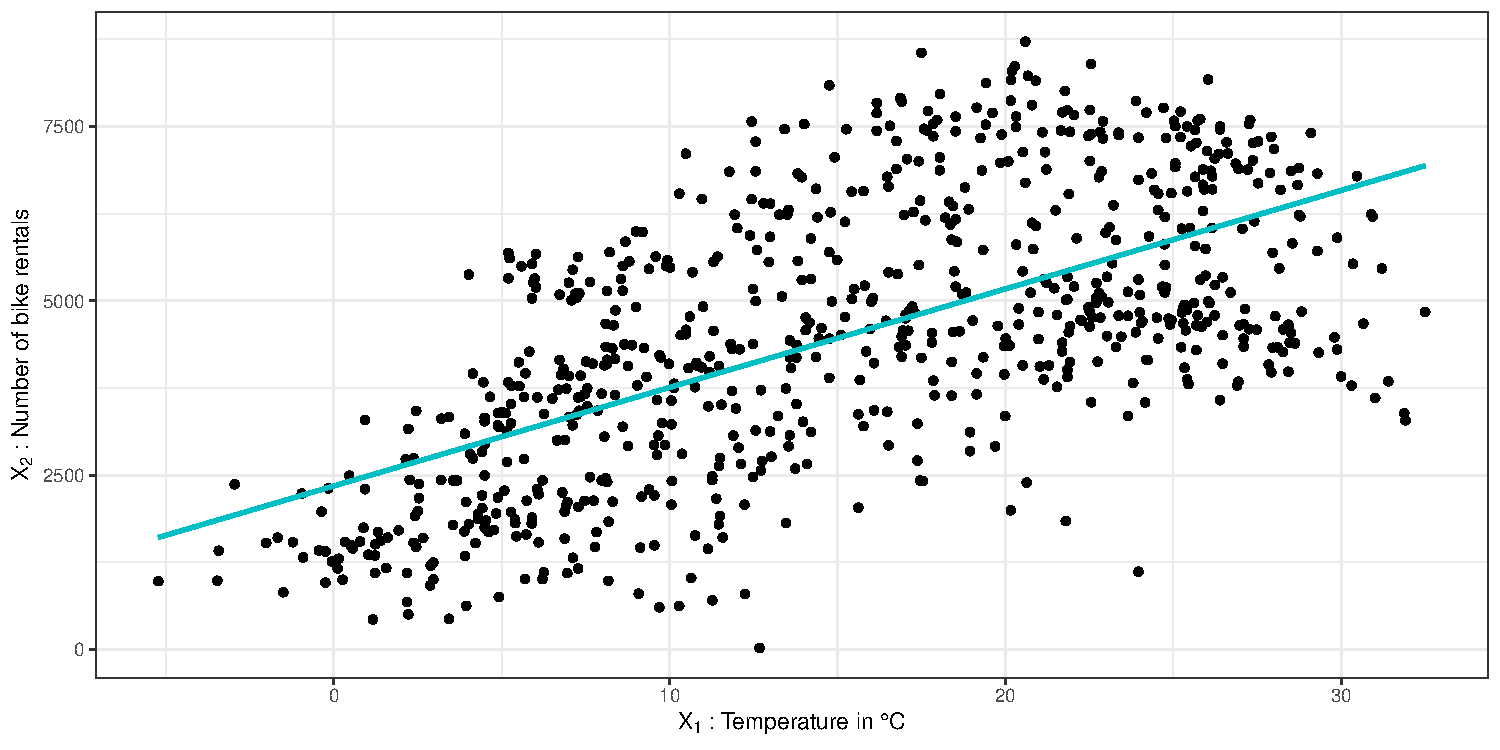
\includegraphics[width = .95\textwidth]{figure/intro_lm_bike.pdf}
            %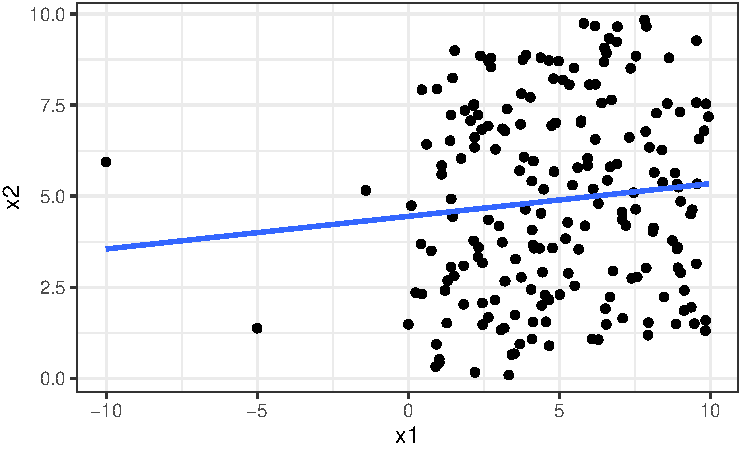
\includegraphics[width = \textwidth]{figure/lm_bad_fit2.pdf}
        \end{center}
    \end{column}
\end{columns}

%\medskip

\only<3->{
\textbf{Idea of GAMs:}

    \begin{itemize}
        \item Instead of linear terms $\theta_j x_j$, use flexible functions $f_j(x_j)$ $\leadsto$ splines
            $$g(\E (y \mid \xv)) = \theta_0 + f_1(x_1) + f_2(x_2) + \ldots + f_p(x_p)$$
    
        \item Preserves additive structure and allows to model non-linear effects
        \item Splines have smoothness param. to control flexibility (prevent overfitting)\\
        $\leadsto$ Needs to be chosen, e.g., via cross-validation
    \end{itemize}}   

\end{frame}


\begin{frame}{Generalized Additive Model (GAM) - Example}
Fit a GAM with smooth splines for four numeric features of bike rental data \\
$\leadsto$ more flexible and better model fit but less interpretable than LM

\begin{columns}[T, totalwidth=\textwidth]
\begin{column}{0.5\textwidth}
\begin{table}[ht]
\centering
\scriptsize
% \begin{tabular}{rrrrr}
%   \hline
%  & edf & Ref.df & F & p-value \\ 
%   \hline
% s(temp) & 5.8 & 7.0 & 57.2 & 0.00 \\ 
%   s(hum) & 4.0 & 5.1 & 68.0 & 0.00 \\ 
%   s(windspeed) & 1.7 & 2.1 & 50.1 & 0.00 \\ 
%   s(days\_since\_2011) & 8.3 & 8.8 & 154.4 & 0.00 \\ 
%   \hline
\begin{tabular}{rrr}
  \hline
 & edf & p-value \\ 
  \hline
s(temp) & 5.8 & 0.00 \\ 
  s(hum) & 4.0 & 0.00 \\ 
  s(windspeed) & 1.7 & 0.00 \\ 
  s(days\_since\_2011) & 8.3 & 0.00 \\ 
   \hline
\end{tabular}
\end{table}


\textbf{Interpretation}
\begin{itemize}
    %\item If the temperature increases by 1 degree Celsius then the log odds of high number of bike rentals increase linearly by 0.3 c.p.
    \item Interpretation is done visually and relative to average prediction
    %, also see PDPs
    \item Edf: effective degrees of freedom\\
    $\leadsto$ represents degree of smoothness/complexity
\end{itemize}
\end{column}
\hfill
\centering
\begin{column}{0.5\textwidth}
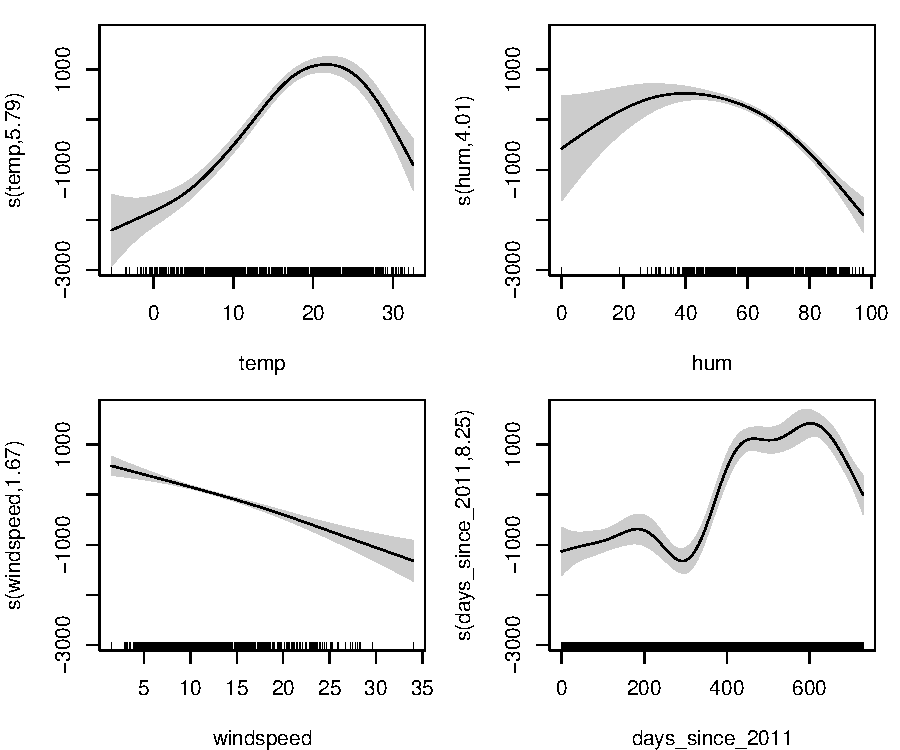
\includegraphics[width = \textwidth]{figure/gam_effects.pdf}
\end{column}
\end{columns}
\end{frame}

%------------------------------------------------------------------
%------------------------------------------------------------------

\begin{frame}{Model-based Boosting % OLD
%\citebutton{Bühlmann, Yu 2003}{https://doi.org/10.1198/016214503000125}
% new
\furtherreading{BÜHLMANNYU2003} % OLD
%\citebutton{Bühlmann, Hothorn 2008}{https://arxiv.org/abs/0804.2752}
% new
\furtherreading{BÜHLMANNHOTHORN2008}}

\begin{itemize}%[<+->]
%\setlength\itemsep{2em}
\item Boosting iteratively combines weak base learners to create powerful ensemble 
\item
Idea: Use simple BLs (e.g. univar., with splines) to ensure interpretability
%$\leadsto$ e.g., linear BL with single features in each iteration
%Boosting with gradient descent using interpretable base learners (e.g., use base learners with single features in each iteration $\leadsto$ coordinate gradient descent)
%The resulting ensemble is also interpretable.
%\pause
\item
Possible to combine BL of same type (with distinct parameters $\thetav$ and $\ts$):
%Two linear base learners $b_j(x, \theta)$ and $b_j(x, \theta^{\star})$ of the same type, but distinct parameter vectors $\theta$ and $\theta^{\star}$ can be combined in a base learner of the same type:
$$\bljt + \bljts = \bl[j](\xv, \thetav + \ts) $$
\pause
\item %In each iteration, a set of BLs is fitted on pseudo residuals. The one with the best fit is added to the previously computed model (using step-size $\nu$), e.g.,
In each iteration, fit a set of BLs, add best one to model (with step-size $\nu$):
%\medskip
\begin{align*}
\fmh[1] &= \hat{f}_0 + \nu \textcolor{blue}{\bl[3](\xv_3, \thetam[1])} \\
\fmh[2] &= \fmh[1] + \nu \textcolor{blue}{\bl[3](\xv_3, \thetam[2])} \\
%= \hat{f}_0 + \nu \textcolor{blue}{b_3(x_3, \theta^{[1]})} + \nu \textcolor{blue}{b_3(x_3, \theta^{[2]})}
\fmh[3] &= \fmh[2] + \nu \textcolor{orange}{\bl[1](\xv_1, \thetam[3])} \\
%= \hat{f}_0 + \nu \textcolor{blue}{b_3(x_3, \theta^{[1]})} + \nu \textcolor{blue}{b_3(x_3, \theta^{[2]})} + \nu \textcolor{orange}{b_1(x_1, \theta^{[3]})} 
&= \hat{f}_0 + \nu \left(\textcolor{blue}{\bl[3](\xv_3, \thetam[1] + \thetam[2])} + \textcolor{orange}{\bl[1](\xv_1, \thetam[3])}\right) 
\\
&= \hat{f}_0 + \textcolor{blue}{\hat{f}_3(\xv_3)} + \textcolor{orange}{\hat{f}_1(\xv_1)}
\end{align*}
\item Final model is additive GAM, we can read off effect curves
\end{itemize}
\end{frame}










\begin{frame}{Model-based Boosting - Linear Example}

Simple case: Use linear model with single feature (including intercept) as BL
$$
\bl[j](x_j, \thetav) = x_j\thetav + \thetav_0 \hspace*{0.2cm}\text{ for } j = 1,\ldots p \hspace*{0.3cm} \leadsto \text{ordinary linear regression}
$$

\begin{itemize}
\item<1-> Here: Interpretation of weights as in LM
\item<1-> After many iterations, it converges to same solution as LM %least square estimate of
\item<2-> Early stopping allows feature selection \& may also prevent\\ overfitting (regularization)
%\item Specifying loss and link function according to exponential family leads a (regularized) GLM
\end{itemize}
\begin{columns}[T, totalwidth=\textwidth]
\begin{column}{0.49\linewidth}
\scriptsize
\begin{table}[ht]
\centering
\tiny
\begin{tabular}{r|r|l}
  %\hline
\textbf{1000 iter. with $\nu = 0.1$} & Intercept & Weights \\ 
  \hline  \hline
days\_since\_2011 & -1791.06 & 4.9 \\ 
  \hline
  hum & 1953.05 & -31.1 \\ 
    \hline
  season & 0 &  \begin{tabular}[c]{@{}l@{}}
  WINTER: -323.4\\
  SPRING: 539.5\\
  SUMMER: -280.2\\
  FALL: 67.2
  \end{tabular}\\
    \hline
  %season &  & WINTER: -323.4, SPRING: 539.5, SUMMER: -280.2, FALL: 67.2 \\ 
  temp & -1839.85 & 120.4 \\ 
    \hline
  windspeed & 725.70 & -56.9 \\ 
    \hline
  offset & 4504.35 &  \\ 
   %\hline
\end{tabular}
\end{table}
% \centering
% $\Rightarrow$ Converges to solution of LM 
\end{column}
\begin{column}{0.49\linewidth}

\only<1>{\scriptsize
\medskip
Relative frequency of selected BLs across iterations
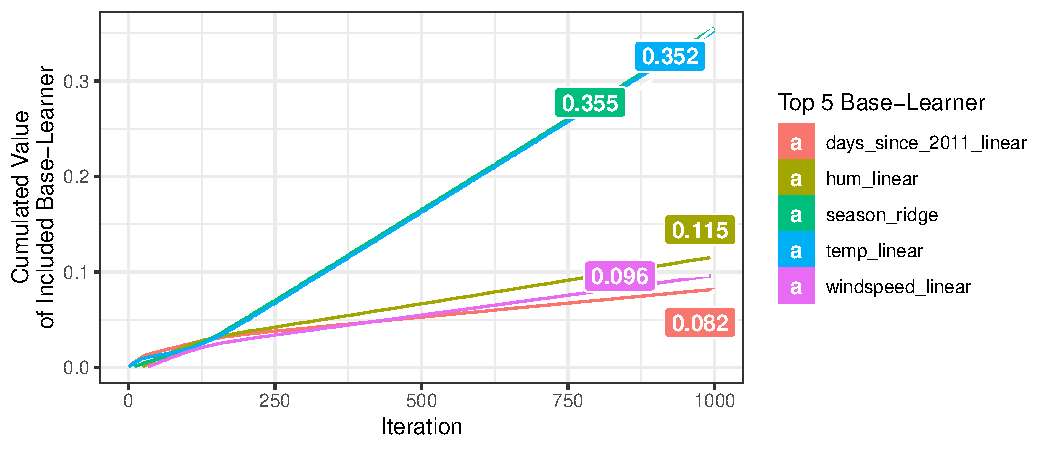
\includegraphics[width = .95 \linewidth]{figure/compboost_base_linear.pdf}}


\only<2>{
\begin{table}[ht]
\centering
\tiny
\begin{tabular}{r|r|l}
  %\hline
 \textbf{20 iter. with $\nu = 0.1$} & Intercept & Weights \\ 
  \hline  \hline
  days\_since\_2011 & -1210.27 & 3.3 \\ 
    \hline
   season & 0 & 
   \begin{tabular}[c]{@{}l@{}}
  WINTER: -276.9\\
  SPRING: 137.6\\
  SUMMER: 112.8\\
  FALL: 20.3
   \end{tabular}\\
     \hline
  temp & -1118.94 & 73.2 \\ 
    \hline
  offset & 4504.35 &  \\ 
   %\hline
\end{tabular}
\end{table}
% \centering
% \scriptsize
% $\Rightarrow$ 3 BLs selected after 20 iter. (feature selection)
}
\end{column}
\end{columns}

\begin{columns}[T, totalwidth=\textwidth]
\begin{column}{0.49\linewidth}
\scriptsize
\centering
$\Rightarrow$ Converges to solution of LM 
\end{column}
\begin{column}{0.49\linewidth}

\only<2>{
\centering
\scriptsize
$\Rightarrow$ 3 BLs selected after 20 iter. (feature selection)
}
\end{column}
\end{columns}
% \begin{itemize}
%     \item Linear base learners for numeric features and categorical base learner for season
%     \item 3 base learners selected after 100 iterations
% \end{itemize}

\end{frame}


\begin{frame}{Linear Example: Interpretation}

\medskip
\textbf{Feature importance:} aggregated change in risk in each iteration per feature
\begin{itemize}
    \item E.g. iter. 1: \code{days\_since\_2011} with risk reduction (MSE) of 140,782.94
    \item For every iteration the change in risk can be attributed to a feature
\end{itemize}
\medskip

\begin{columns}[T, totalwidth=\textwidth]
\begin{column}{0.47\linewidth}
\hspace{46pt}{\scriptsize{1000 iterations}}
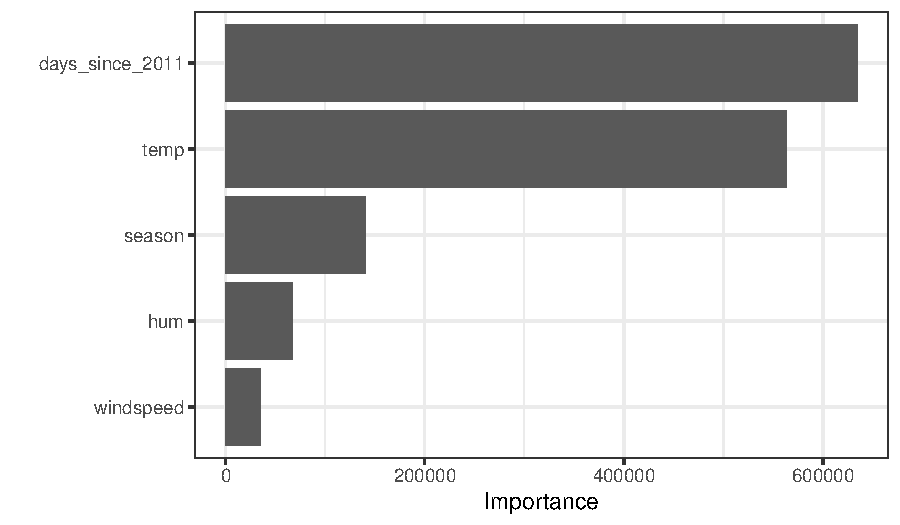
\includegraphics[width = \linewidth]{figure/compboost_pfi_base2.pdf}\\
\centering \scriptsize
In-bag-risk: 434,686.0 \\
OOB risk (10-fold CV): 446,450.0
\end{column}


\begin{column}{0.47\linewidth}
\hspace{46pt}{\scriptsize{20 iterations}}
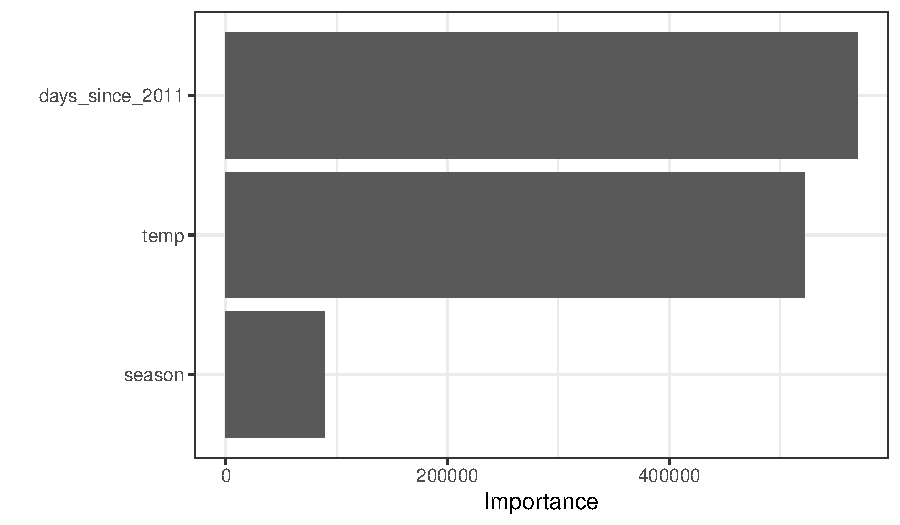
\includegraphics[width = \linewidth]{figure/compboost_pfi_base1.pdf}\\
\centering \scriptsize
In-bag-risk: 693,505.0\\
OOB risk (10-fold CV): 705,776.0
\end{column}
\end{columns}

\begin{center}
\scriptsize
$\Rightarrow$ Difference in risk: 258,819.0\\
Difference in OOB risk: 259,326.0\\
% \normalsize
% \medskip
% $\leadsto$ Ranking of features stays the same

\end{center}

\end{frame}


\begin{frame}{Non-linear Example: Interpretation}

\begin{itemize}
    \item Fit model on bike data with different BL types (1000 iter.) % OLD
%\citebutton{Daniel Schalk et al. 2018}{https://doi.org/10.21105/joss.00967}
% new
\furtherreading{SCHALKETAL2018}
    \item BLs: linear and centered splines for numeric feat., categorical for season
    %and categorical base learner for season
\end{itemize}
\begin{columns}[T, totalwidth = \textwidth]
\visible<2->{
\begin{column}{0.5\linewidth}
\hspace{45pt}{\scriptsize{Feature importance}}
 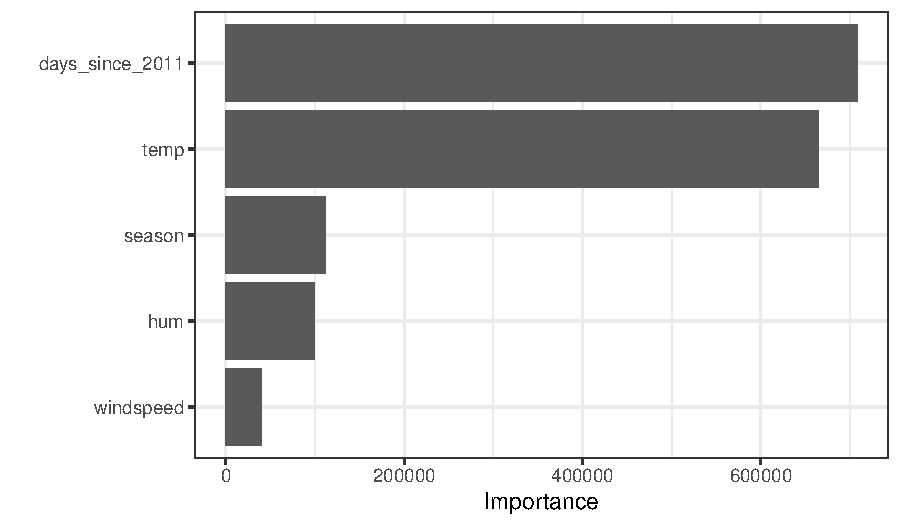
\includegraphics[width = \linewidth]{figure/compboost_pfi.pdf}
%Feature importance (risk reduction over iter.)\\
%$\leadsto$ \code{days\_since\_2011} most important
%\scriptsize
%\verbatiminput{figure/mboost_output.txt}
\end{column}
}
\visible<2->{
\begin{column}{0.5\linewidth}  %%<--- here
\hspace{23pt}{\scriptsize{Feature effect}}
  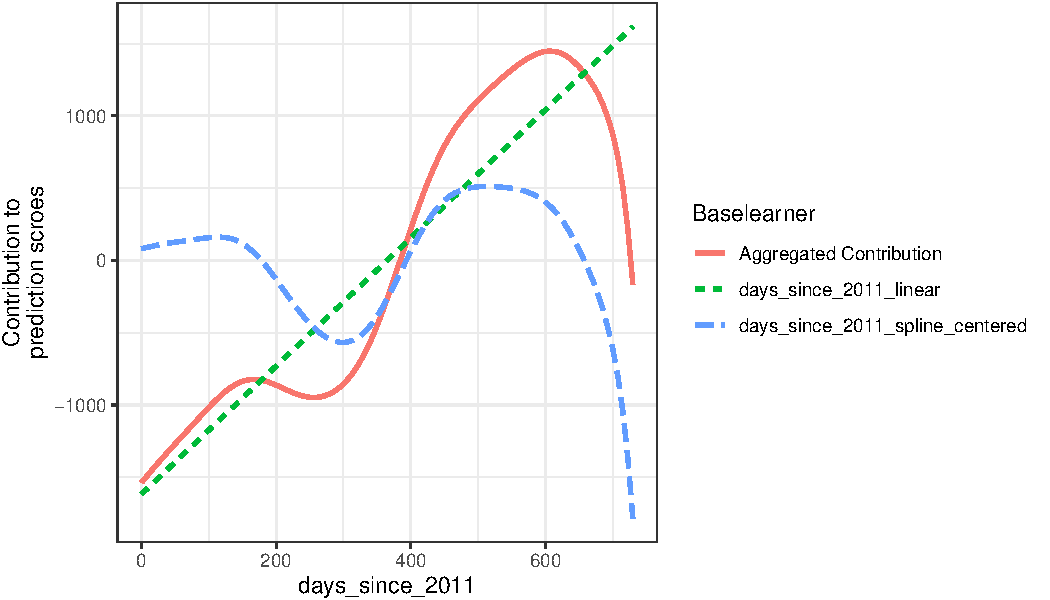
\includegraphics[width = \linewidth]{figure/compboost_pfe.pdf}
%Partial feature effect for \code{days\_since\_2011}\\
%$\leadsto$ Total effect: Combination of partial effects of linear BL and centered spline BL
\end{column}
}
\end{columns}
\smallskip
\scriptsize
\only<2->{\qquad $\Rightarrow$ In-bag-risk: 250,202.0 \, ; \, OOB risk (10-fold CV): 267,497.0 (difference to lin. example: 178,953.0)\\
\qquad $\Rightarrow$ In-bag-risk: 434,686.0 \, ; \, OOB risk (10-fold CV): 446,450.0 (previous lin. example with 1000 iter.)}
\begin{itemize}
    \normalsize
    \item<2->  Feature importance (risk reduction over iter.) \\ $\leadsto$ \code{days\_since\_2011} most important
    \item<2-> Total effect for \code{days\_since\_2011}\\
$\leadsto$ Combination of partial effects of linear BL and centered spline BL
\end{itemize}
\end{frame}

%------------------------------------------------------------------
%------------------------------------------------------------------


% \begin{frame}{Decision Trees}

% \begin{columns}[totalwidth=\textwidth]

% \begin{column}{0.3\textwidth}

%   \begin{tikzpicture}
%   \usetikzlibrary{arrows}
%     \usetikzlibrary{shapes}
%      \tikzset{treenode/.style={draw, circle, font=\small}}
%      \tikzset{line/.style={draw, thick}}
%      \node [treenode, draw=red] (a0) {$a_0$};
%      \node [treenode, below=0.75cm of a0, xshift=-1cm]  (a1) {$a_1$};
%      \node [treenode, draw=red, below=0.75cm of a0, xshift=1cm]  (a2) {$a_2$};

%      \node [treenode, draw=red, below=0.75cm of a2, xshift=-1cm] (a3) {$a_3$};
%      \node [treenode, below=0.75cm of a2, xshift=1cm]  (a4) {$a_4$};

%      \node [treenode, below=0.75cm of a3, xshift=-1cm] (a5) {$a_5$};
%      \node [treenode, below=0.75cm of a3, xshift=1cm]  (a6) {$a_6$};

%      \path [line] (a0.south) -- + (0,-0.4cm) -| (a1.north) node [midway, above] {$x_1<0.3$};
%      \path [line] (a0.south) -- +(0,-0.4cm) -|  (a2.north) node [midway, above] {$x_1\geq0.3$};

%      \path [line] (a2.south) -- + (0,-0.4cm) -| (a3.north) node [midway, above] {$x_1<0.6$};;
%      \path [line] (a2.south) -- +(0,-0.4cm) -|  (a4.north) node [midway, above] {$x_1\geq0.6$};


%      \path [line] (a3.south) -- + (0,-0.4cm) -| (a5.north) node [midway, above] {$x_2<0.2$};;
%      \path [line] (a3.south) -- +(0,-0.4cm) -|  (a6.north) node [midway, above] {$x_2\geq0.2$};

%   \end{tikzpicture}

% \end{column}

% \begin{column}{0.7\textwidth}

% Properties:
% \begin{itemize}
%     \item able to model non-linear effects
%     \item terminal nodes (aka leaf nodes) can have several observations and predicts the mean outcome over these
%     \item Applicable to regression and classification
% \end{itemize}

% Interpretation:
% \begin{itemize}
%     \item directly by following the tree (i.e., sequence of rules)
%     \item Feature importance by (scaled) score of much the splitting criterion was reduced compared to the parent
% \end{itemize}

% \end{column}

% \end{columns}

% \end{frame}

% \begin{frame}{Decision Trees % OLD
%\citebutton{Breiman et al. (1984)}{https://doi.org/10.1201/9781315139470}
% new
% \furtherreading{BREIMANETAL1984}}

% %\textbf{Problem}: Can we model non-linear effects and interactions automatically (without manual specification as in GLMs or GAMs)?\\
% %Relationship between features and target are non-linear or interactions are present\\
% %\medskip
% %\pause

% \begin{columns}[T, totalwidth=\textwidth]

% \begin{column}{0.7\textwidth}
% \textbf{Idea of decision trees}: 
% %Split data in different subsets based on cut-off values in features 
% Partition data into subsets based on cut-off values in features (found by minimizing a split criterion via greedy search) and predict constant mean $c_m$ in leaf node $\mathcal{R}_m$:

% $$
% \hat f(x) = \sum_{m=1}^M c_m \mathds{1}_{\{x \in \mathcal{R}_m\}}
% $$

% % \begin{itemize}
% % \item where $c_m$ is a constant and 
% % \item $\mathcal{R}_m$ the $m$-th leaf node of the tree
% % \end{itemize}
% \pause
% \begin{itemize}
%     %\item Finding best split point (CART): Greedy search for the point that minimizes the variance of $y$ (regression) or the Gini index (classification)
%     \item Applicable to regression and classification
%     \item Able to model interactions and non-linear effects
%     \item Able to handle mixed feature spaces and missing values
% \end{itemize}

% \end{column}
% \begin{column}{0.3\textwidth}

% \begin{tikzpicture}[scale=0.75, transform shape]
%    \usetikzlibrary{arrows}
%     \usetikzlibrary{shapes}
%      \tikzset{treenode/.style={draw, circle, font=\small}}
%      \tikzset{line/.style={draw, thick}}
%      \node [treenode, draw=red] (a0) {};
%      \node [treenode, below=0.75cm of a0, xshift=-1.5cm]  (a1) {};
%      \node [treenode, below=0.75cm of a0, xshift=1.5cm]  (a2) {};

%      \node [treenode, below=0.75cm of a2, xshift=-0.75cm] (a3) {$c_1$};
%      \node [treenode, below=0.75cm of a2, xshift=0.75cm]  (a4) {$c_2$};

%     \node [treenode, below=0.75cm of a1, xshift=-0.75cm] (a5) {$c_3$};
%     \node [treenode, below=0.75cm of a1, xshift=0.75cm]  (a6) {$c_4$};

%      \path [line] (a0.south) -- + (0,-0.4cm) -| (a1.north) node [midway, above] {$x_1<3$};
%      \path [line] (a0.south) -- +(0,-0.4cm) -|  (a2.north) node [midway, above] {$x_1\geq3$};

%      \path [line] (a2.south) -- + (0,-0.4cm) -| (a3.north) node [midway, above] {$x_2<6$};;
%      \path [line] (a2.south) -- +(0,-0.4cm) -|  (a4.north) node [midway, above] {$x_2\geq6$};

%     \path [line] (a1.south) -- + (0,-0.4cm) -| (a5.north) node [midway, above] {$x_3<2$};;
%     \path [line] (a1.south) -- +(0,-0.4cm) -|  (a6.north) node [midway, above] {$x_3\geq2$};

%     %\path (a5.south) -- +(0,0) -|  (a5.south) node [midway, below] {$f_{1,3}(x_1,x_3)$};
%     %\path (a6.south) -- +(0,0) -|  (a6.south) node [midway, below] {$f_{1,3}(x_1,x_3)$};

%     %\path (a3.south) -- +(0,0) -|  (a3.south) node [midway, below] {$f_{1,2}(x_1,x_2)$};
%     %\path (a3.south) -- +(0,0) -|  (a4.south) node [midway, below] {$f_{1,2}(x_1,x_2)$};
%     % \path (a3) edge [bend right, draw=white] node [below] {$f_{1,2}(x_1,x_2)$} (a4);
%     % \path (a5) edge [bend right, draw=white] node [below] {$f_{1,3}(x_1,x_3)$} (a6);
%    \end{tikzpicture}
   
% \end{column}
% \end{columns}

% \medskip
% \pause
% \textbf{Interpretation}
% \begin{itemize}
%     \item Directly by following the tree structure (i.e., sequence of decision rules)
%     \item Importance of $x_j$: Aggregate ``improvement in split criterion'' over all splits where $x_j$ was involved\\
%     (e.g., variance for regression or Gini index for classification)
%     %Feature importance: How much did split criterion improve compared to parent node% by (scaled) score of how much splitting criterion (e.g. variance) is reduced compared to a parent node
% \end{itemize}



% \end{frame}

% \begin{frame}{Decision Trees - Example}
% \begin{itemize}
%     \item Fit decision tree with tree depth of 3 on bike data
%     \item E.g., mean prediction for the first 105 days since 2011 is 1798 (applies to $\hat = 15\%$ of the data)
%     \item \code{days\_since\_2011} shows highest feature importance (explains most of variance)
% \end{itemize}
% \begin{columns}[T, totalwidth=\textwidth]
% \begin{column}{0.4\textwidth}
% \vspace{1.5cm}
% \begin{table}[ht]
% \centering
% \begin{tabular}{lr}
%   \hline
%  Feature & Importance \\
%   \hline
% days\_since\_2011 & 79.53 \\ 
%   temp & 17.55 \\ 
%   hum & 2.92 \\ 
%    \hline
% \end{tabular}
% \end{table}
% \end{column}
% \begin{column}{0.6\textwidth}
%   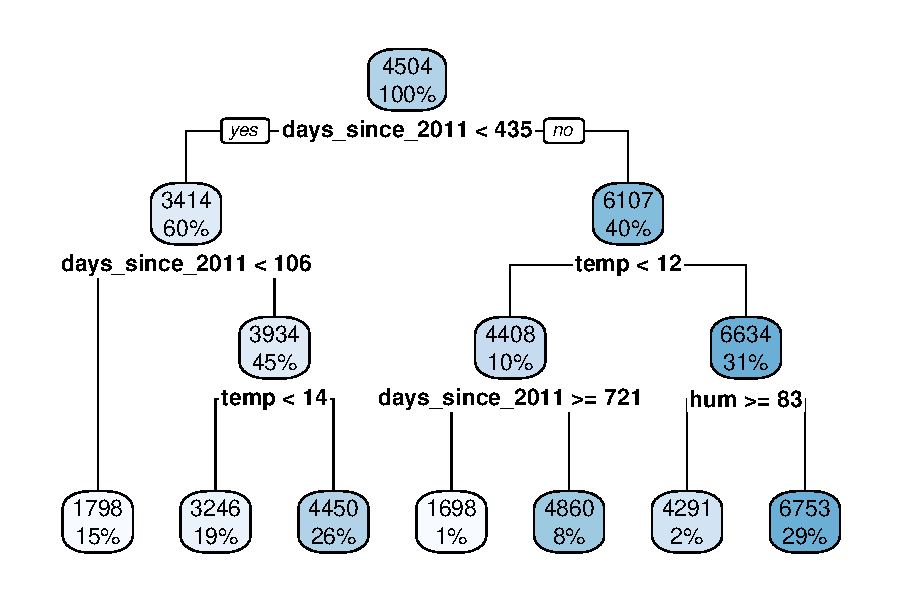
\includegraphics[width = \textwidth]{figure/tree.pdf} 
% \end{column}
% \end{columns}
 
% \end{frame}
% %------------------------------------------------------------------
% %------------------------------------------------------------------

% %\begin{frame}[c]{Decision Rules}

% %\texttt{IF COND$_1$ AND COND$_2$ AND ... THEN value}

% %\begin{itemize}
% %    \item \texttt{COND$_i$} can be of the form \texttt{feature <op> value} where \texttt{<op>} can be for example $\{=, <, > \}$
% %\end{itemize}

% %\pause
% %\medskip

% %Properties:
% %\begin{description}
% %    \item{Support} Fraction of observations to support appliance of rule
% %    \item{Accuracy} for predicting the correct class under the condition(s)
% %\end{description}

% %$\leadsto$ often trade-off between these two

% %\pause
% %\medskip

% %$\leadsto$ many different ways to learn a set of rules (incl. a default rule if none of the rules are met)

% %\end{frame}

% %------------------------------------------------------------------
% %------------------------------------------------------------------


% \begin{frame}{Other Interpretable Models}

% \begin{columns}[totalwidth=\textwidth]
%     \begin{column}{0.7\textwidth}
%         \textbf{RuleFit} % OLD
%\citebutton{Friedman and Popescu 2008}{https://arxiv.org/abs/0811.1679}
% new
% \furtherreading{FRIEDMANPOPESCU2008}
%         \begin{itemize}
%             \item Combination of linear models and decision trees 
%             \item Allows for feature interactions and non-linearities
%         \end{itemize}

%         \only<2->{\textbf{Decision Rules} % OLD
%\citebutton{Holte 1993}{https://doi.org/10.1023/A:1022631118932}
% new
% \furtherreading{HOLTE1993}
%         \begin{itemize}
%             \item Simple ``if -- then'' statements - very intuitive and easy-to-interpret
%             \item Most methods work only for classification and categorical feat.
%         \end{itemize}}

%         \only<3->{\textbf{Naive Bayes}
%         % OLD
%\citebutton{Zhang 2004}{https://www.aaai.org/Papers/FLAIRS/2004/Flairs04-097.pdf}
% new
% \furtherreading{ZHANG2004}
%         %$$P (C_k \mid x ) = \frac{1}{Z} P(C_k) \prod_{i=1}^{n} P(x_i \mid C_k) $$
%         \begin{itemize}
%             \item Uses Bayes' theorem to assign class prob. to observations
%             %Product of (conditional) probabilities for a class on the value of each feature
%             %For each feature, it calculates the probability for a class depending on the value of the feature. 
%             \item Strong assumption: Independence of features
%         \end{itemize}}

%         \only<4->{\textbf{k-Nearest Neighbor}
%         % OLD
%\citebutton{Cover 1967}{https://doi.org/10.1109/TIT.1967.1053964}
% new
% \furtherreading{COVER1967}
%         \begin{itemize}
%             \item (Closely related to case-based reasoning)
%             \item Average of the outcome of neighbors -- local explanation
%         \end{itemize}

%         ...}
%     \end{column}
%     \begin{column}{0.3\textwidth}
%     \vspace{\dimexpr-2\parsep-2\parskip\relax}
%         \begin{center}
%             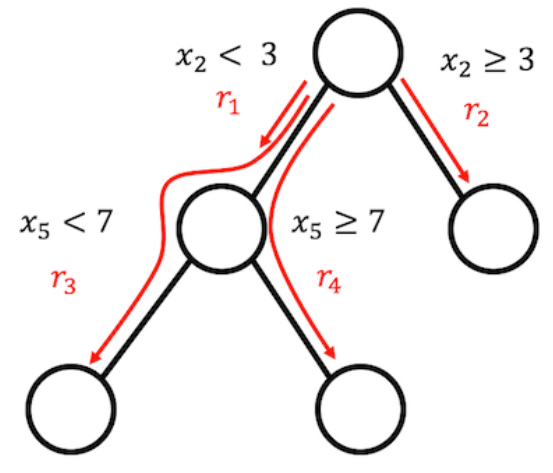
\includegraphics[width = 0.6\textwidth]{figure/RuleFit.png} \\
%             \smallskip
%             \only<2->{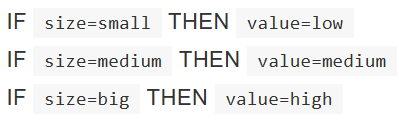
\includegraphics[width = 0.8\textwidth]{figure/decision_rules.png} \\
%             % OLD
%\citebutton{Molnar 2022}{https://christophm.github.io/interpretable-ml-book/}
% new
% \furtherreading{MOLNAR2022}\\
%             \smallskip}
%             \only<4->{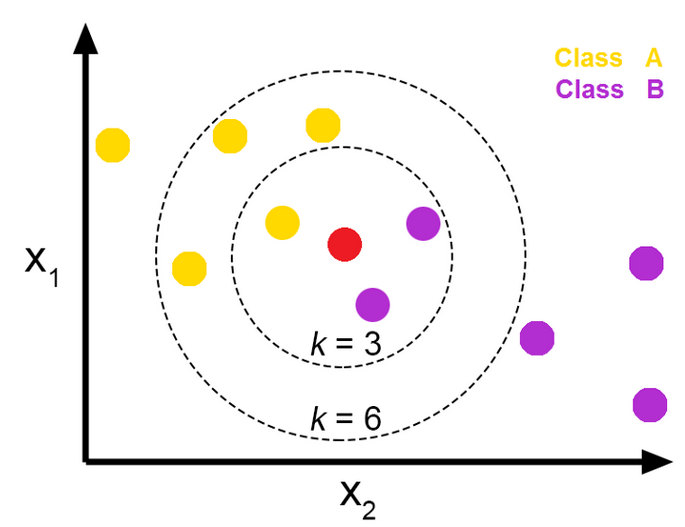
\includegraphics[width = 0.7\textwidth]{figure/knn.png} 
%             % OLD
%\citebutton{José 2018}{https://towardsdatascience.com/knn-k-nearest-neighbors-1-a4707b24bd1d}
% new
% \furtherreading{JOS2018}}
%         \end{center}
%     \end{column}
% \end{columns}

% \end{frame}


\endlecture
\end{document}
